\chapter{モニタ}
\label{monitor}
複数のプロセス(スレッド)で資源を共有する際に,
プロセスの同期や相互排除にセマフォを用いることを既に学んだ.
しかし,
セマフォは基本的な機能を提供するだけで使い方はプログラマ任せなので,
間違った使用がされる可能性が高い.
その結果,
タイミングに依存した発見の難しいバグを持ったプログラムが作成される.
そこで,プログラミング言語と一体になり\footnote{
  本章の話題はオペレーティングシステムではなくプログラミング言語である.},
プログラマに同期機構を強制的に利用させる仕組みが考案された.
そのような仕組みの一つとして\emph{モニタ(Monitor)}を紹介する.

%==============================================================================
\section{概要}
モニタはリソース管理用の機能と制約を持った
\emph{抽象データ型}\cite{AbstractDataType}である.
C++やJavaなどを学んだことのある人なら,
「抽象データ型はクラスのこと」と言えば分かりやすいと思われる.

モニタは抽象データ型の一種であるが,
プロセス(スレッド)間の同期を行う機構が予め組込まれ,
その制約の下で使用するものである.
モニタの特長を以下に箇条書きにする.

\begin{itemize}
\item プログラマが定義できる型である.(抽象データ型で一般的)
\item データと操作をまとめて定義する.(抽象データ型で一般的)
\item 同期のための機能が組込まれている.(モニタ独特)
\end{itemize}

なお,Javaのクラスは同期のための機構も持っており,
一定のルールに従って使用すればモニタに近い使用もできる.
モニタをサポートするプログラミング言語は Concurrent Pascal が有名である.

%==============================================================================
\section{構成要素}
モニタは次の要素を持つ抽象データ型である.
\figref{monitor}にモニタの模式図\footnote{
  \figref{monitor}では,初期化プログラムが省略してある.}を示す.

\begin{itemize}
\item 資源(データ,変数)
\item 手続き(操作,メソッド)
\item ガード
\item 条件変数
\end{itemize}

\begin{myfig}{btp}{モニタの模式図}{monitor}
  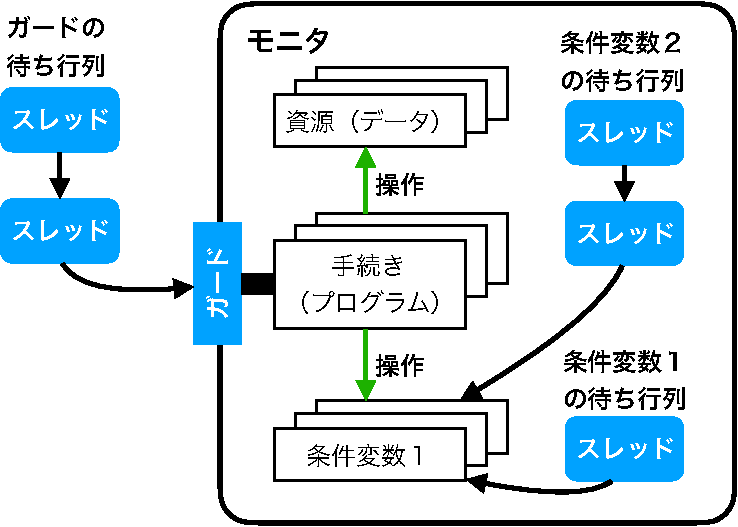
\includegraphics[scale=0.6]{Fig/monitor-crop.pdf}
\end{myfig}

\subsection{資源(データ,変数)}
複数のスレッドによって共有される変数のことである.
モニタの内部に必要に応じて名前付きで宣言する.
モニタの外から直接アクセスすることはできない.

\subsection{手続き(操作,メソッド)}
外部から呼び出されるプログラムである.
モニタの内部に必要に応じて名前付きで定義する.
モニタの外部から資源にアクセスできるインタフェースは手続きだけである.
手続きの実行は\emph{ガード}の働きにより排他的に行われ,
同時に実行される手続きは必ず一つ以内である.

\subsection{ガード}
モニタに一つのガードが存在し,
手続きを排他的に実行するために用いられる.
手続きを実行するときは自動的にガードにロックがかけられる.
複数のスレッドが同時にモニタに入ることはできない.
%これにより複数のスレッドが同時にモニタの手続きを実行しないようにする.

\subsection{条件変数}
モニタの内部に必要に応じて名前付きで宣言する.
モニタの外部から直接アクセスすることはできない.
条件変数にはwaitとsignalの二つの操作ができる.
wait操作を行ったスレッドは\emph{ガードを外して}条件変数の待ち行列に入る.
signal操作は条件変数の待ち行列から一つのスレッドを選んで実行可能にする.
実行可能になったスレッドは\emph{ただちに}実行を再開する.
待ち行列にスレッドが複数ある時,
どのスレッドが実行可能になるか明確な決まりはない.

\subsection{初期化プログラム}
モニタのインスタンスを作成する時に,
初期化のために実行されるプログラムである.

%==============================================================================
\section{相互排除問題の解}
前出の架空の銀行口座管理プログラムの例をモニタに置換える.
残高がスレッド間で共有される変数である.
共有変数をスレッド間で安全に共有させるためにモニタを用いる.

\subsection{共有変数の記述}
リスト\ref{monAccount}にJava風の仮想言語による銀行口座の記述を示す.
本物の口座は他にも情報を持っているだろうが,
ここでは口座は残高だけ持っていることにする.

\lstinputlisting[numbers=left,float=btp,label=monAccount,
  caption=モニタによる相互排除の実現(仮想言語版)]{Lst/MonAccount.jama}

\begin{description}
\item [2行]
  この仮想言語では,Javaの class 定義に似た monitor 定義ができるものとする.
\item [3〜4行]
  \emph{資源}の例である.
  この例では残高を表すスレッド間の共有変数(\texttt{money})が資源である.
\item [5〜8行]
  \emph{初期化プログラム}の例である.
  モニタのインスタンス生成時に残高を引数で初期化する.
\item [9〜15行]
  \emph{手続き}の例である.
  手続きは共有資源を書換えるので\emph{クリティカルセクション}であるが,
  自動的に\emph{ガード}をロックし排他的に実行されるので
  \emph{明示的な相互排除を行う必要はない}.
\end{description}

\subsection{共有変数の利用}
リスト\ref{monAccountMain}に,
リスト\ref{monAccount}で定義した\|MonAccount|モニタを
利用した相互排除問題の解を示す.

\lstinputlisting[numbers=left,float=btp,label=monAccountMain,
  caption=モニタによる相互排除の利用(仮想言語版)]{Lst/MonAccountMain.jama}

\begin{description}
\item [2行]
  リスト\ref{monAccount}に示した\|MonAccount|モニタ型のインスタンスを生成する.
\item [3〜8行]
  入金管理スレッドが実行するメソッドである.
  入金額を受信し口座に入金する.
\item [9〜13行]
  引落し管理スレッドが実行するメソッドである.
  支払い金額を受信し口座から引落す.
\item [14〜17行]
  プログラムは\|main()|から実行を開始する.
  \|main()|では「入金管理スレッド」と「引落し管理スレッド」を起動する.
  これらのスレッドがそれぞれ,
  \|receiveThread()|メソッドと\|payThread()|メソッドを実行するものとする.
\end{description}

%==============================================================================
\section{生産者と消費者問題の解}
この問題で\emph{資源}はデータを保管するFIFO構造のバッファである.
このバッファを以下では\emph{キュー}と呼ぶことにする.
キューとキューを操作する手続きは,
全てモニタの中にまとめられる.
キューを使用するユーザプログラムには,
排他や同期に関わる難しいプログラムが含まれない.
資源の操作に関する難しいプログラムが一箇所にまとめられることも,
モニタを使用するメリットである.

以下では生産者と消費者問題の解を示すために,
まず,データのバッファになるキューをモニタを用いて記述する.
次に,キューを使用する生産者スレッドと消費者スレッド作る.

\subsection{キューの記述}
リスト\ref{monProducerConsumer}に
Java風の仮想言語によるキューの記述例を示す.

\lstinputlisting[numbers=left,float=btp,label=monProducerConsumer,
  caption=モニタによるキューの実現(仮想言語版)]{Lst/BoundedBuffer.jama}

\begin{description}
\item [1行] この仮想言語では,
  Javaの\|class|定義に似た\|monitor|定義ができるものとする.
\item [2〜5行] \emph{資源}の例である.
  キューとして使用するリングバッファのデータ構造を宣言している.
  このモニタの目的は,資源であるキューを管理することである.
  手続きを介すること無しに資源にアクセスすることは禁止なので,
  モニタの外部からこれらのデータにアクセスできない.
  \|N|がバッファの大きさ,
  \|buf|がバッファ本体,
  \|first|がバッファ中の次のデータ読みだし位置,
  \|last|がバッファ中の次のデータ書込み位置,
  \|cnt|がバッファ中のデータ件数を表す.
\item [6〜8行] \emph{条件変数}の例である.
  この仮想言語では,\|Condition|型の変数として条件変数を宣言する.
  \|empty|は,
  キューが空の時にデータを取り出そうとしたスレッドが,
  キューにデータが書き込まれるまで待つために使用する条件変数である.
  \|full|は,
  キューが満杯の時にデータを書き込もうとしたスレッドが,
  キューに空きができるまで待つために使用する条件変数である.
\item [9〜14行] \emph{初期化プログラム}の例である.
  モニタのインスタンスを作る際に実行されるものとする.
  引数はバッファの大きさである.
\item [15〜30行] \emph{手続き}の例である.
  手続きはモニタの外部から呼び出すことができる.
  \|append()|はキューにデータを追加する.
  \|remove()|はキューからデータを取り出す.
  これらのプログラムが実行される時は\emph{ガード}による排他制御がされる.
  次にバッファが満杯で待ちが発生する例を考える.

  データをキューに追加するために\|append()|を呼び出したスレッドは,
  コメントに\|(1)|と記された行を実行し,
  キューが満杯の時17行の\|full.wait()|で待ち状態になる.
  待ち状態になる時はガードを外すので,
  他のスレッドがモニタに入ることができる.

  他のスレッドがデータをキューから取り出すために\|remove()|を呼び出すと,
  \|(2)|の行が実行され28行の\|full.signal()|まで進む.
  \|full.signal()|が実行されると待ち状態のスレッドが一つ起床し,
  \|(3)|の行が\emph{ただちに}実行される.
  \|(3)|の実行が終了した後に(4)の行が実行される.
  \|(2)|から\|(4)|の実行の間,
  \emph{ガードは外さないので他のスレッドがモニタに入ることはない.}
\end{description}

\subsection{生産者と消費者スレッドの記述}
リスト\ref{monProducerConsumerMain}に
Java風の仮想言語による生産者と消費者問題の解を示す.
このプログラムはリスト\ref{monProducerConsumer}で定義したキューを使用する.

\lstinputlisting[numbers=left,float=btp,label=monProducerConsumerMain,
  caption=モニタによる生産者と消費者問題の解(仮想言語版)]
                {Lst/BoundedBufferMain.jama}

\begin{description}
\item [2行] 
  リスト\ref{monProducerConsumer}に示した
  \|BoundedBuffer|モニタ型のインスタンスである.
\item [3〜8行]
  生産者スレッドが実行するメソッドである.
  無限にデータを生産し\|queue|に追加し続ける.
\item [9〜14行]
  消費者スレッドが実行するメソッドである.
  \|queue|からデータを取出し処理することを無限に繰り返す.
\item [15〜18行]
  プログラムは\|main()|から実行を開始する.
  \|main()|では「生産者スレッド」と「消費者スレッド」を起動する.
  これらのスレッドがそれぞれ,
  \|producer()|メソッドと\|consumer()|メソッドを実行する.
\end{description}

%==============================================================================
\section{Javaのセマフォクラスによるモニタの実装}
モニタの仕組みをより正確に理解するために,
セマフォによるモニタの実装方法を考えてみる.
リスト\ref{monProducerConsumer}の仮想言語で記述されたモニタを
Javaクラスに書換えたものを
リスト\ref{semProducerBuffer1}とリスト\ref{semProducerBuffer2}に示す.

\lstinputlisting[firstline=3,lastline=36,numbers=left,float=btp,
  label=semProducerBuffer1,
  caption=モニタと同等なキューをセマフォで実現(Java版,前半)]
                {SampleCode/SemBoundedBuffer/SemBoundedBuffer.java}

\lstinputlisting[firstline=37,firstnumber=last,numbers=left,float=btp,
  label=semProducerBuffer2,
  caption=モニタと同等なキューをセマフォで実現(Java版,後半)]
                {SampleCode/SemBoundedBuffer/SemBoundedBuffer.java}

\subsection{モニタ機能のJavaによる実装}
リスト\ref{semProducerBuffer1}は,
モニタと同等な動作をする\|SemBoundedBuffer|クラスである.

\begin{description}
\item [1行]
  \|java.util.concurrent|パッケージの\|Semaphore|クラスを使用する.
  \|Semaphore|クラスはカウンティングセマフォ型である.
\item [2行]
  セマフォを使用したキュークラスを\|SemBoundedBuffer|と名付ける.
\item [3行]
  セマフォ(\|guard|)はモニタのガードの役割りを持っている.
  スレッドは,
  モニタ(\|SemBoundedBuffer|クラス)内の手続き(メソッド)を
  実行する前に\|guard|をロックする.
\item [4〜5行]
  モニタの条件変数に\|signal()|操作を行った時,
  条件変数で待っていたスレッドがあれば\emph{ただちに}実行しなければならない.
  待っていたスレッドを先に実行させるために,
  \|signal()|操作を行ったスレッドを待ちにするセマフォ(\|next|)と
  \|next|を待っているスレッドの数を記憶する変数(\|nextCont|)を準備する.
\item [6行]
  \emph{条件変数型}(\|Condition|)を内部クラスとして定義する.
\item [7〜8行]
  条件変数にwait操作を行った時に
  スレッドを待ち状態にするためのセマフォ(\|sem|)と
  待っているスレッドの数をカウントする変数(\|count|)である.
\item [9行]
  \|await()|は条件変数のwait操作を行うメソッドである.
  Javaの\|Object|クラスに別の\|wait()|メソッドが定義さているので,
  名前を\|await|にした.
\item [11〜15行]
  \|release()|はセマフォにV操作を行う.
  %\|Semaphore|クラスのインスタンスメソッドである.
  \|nextCont|は\|signal()|中で待っているスレッドの数である.
  待っているスレッドがある場合は起こす.
  そうでなければモニタのガードを外す.
\item [16行]
  \|acquireUninterruptibly()|はセマフォにP操作を行う.
  %\|Semaphore|クラスのインスタンスメソッドである.
  \|sem|は初期値0のセマフォなので,
  \|await()|を呼び出したスレッドがここでブロックする.
\item [19行]
  条件変数にsignal操作を行うメソッドである.
\item [20〜25行]
  条件変数を待っているスレッドの数(\|count|)を調べ,
  1以上なら22行で起床させる.
  自身は23行でブロックし,
  起床したスレッドが\|exitProc()|を実行しモニタを出るのを待つ.
\item [28行]
  モニタ手続きの最後の行で呼び出すメソッドである.
  \|signal()|中の23行でブロックしているスレッドがあれば起床させる.
  なければモニタのガードを外す.
\end{description}

\subsection{モニタ機能の使用}
リスト\ref{semProducerBuffer2}に\|SemBoundedBuffer|クラスの後半を示す.
ここでは,\|SemBoundedBuffer|クラスの前半で定義したモニタ機能を使用している.

\begin{description}
\item [35〜38行]
  \emph{資源}(リングバッファ)を表現するための変数を宣言する.
  モニタ(クラス)の外部から資源を隠蔽するために
  \|private|修飾子を付けて宣言する.
\item [39〜41行]
  \emph{条件変数}は
  前半で定義した\|Condition|クラスのインスタンス変数である.
\item [42〜47行]
  \emph{初期化}はクラスのコンストラクタとして実装する.
\item [48〜67行]
  \emph{手続き}は仮想言語で定義したものに,
  50行と59行の「ガード取得」,
  56行と65行の「手続きの出口処理」が追加されている.
\end{description}

%==============================================================================
\section{Javaのモニタ風機構による生産者と消費者問題の解}
Java言語はモニタに似た同期機構をサポートしている.
リスト\ref{javaMonProducerConsumer}に
Javaによる生産者と消費者問題の解を示す.
Javaには\emph{条件変数}に相当するものが無い.

\lstinputlisting[numbers=left,float=btp,label=javaMonProducerConsumer,
  caption=Javaのモニタ風機構による生産者と消費者問題の解]
                {SampleCode/MonBoundedBuffer/MonBoundedBuffer.java}

\begin{description}
\item [1行]
  Javaのモニタ風機構を利用したキュークラスを\|MonBoundedBuffer|と名付ける.
\item [2〜5行]
  \emph{資源}(リングバッファ)を表現するための変数を宣言する.
  クラスの外部から資源を隠蔽するために\|private|修飾子を付けて宣言する.
\item [6〜11行]
  \emph{初期化}をコンストラクタとして実装する.
\item [13行]
  クラスの内部だけで呼び出す\|private|なメソッドである.
  \|await()|メソッドは条件変数の\|wait()|に似た働きをする.
\item [14行]
  \|await()|メソッドは\|Object|クラスの\|wait()|メソッドを呼び出す.
  Javaオブジェクトは暗黙の条件変数が一つあるような構造になっている.
  \|wait()|メソッドは暗黙の条件変数の待ち行列\footnote{
    Javaでは待機セットと呼ぶ.}にスレッドを入れる.
  \|wait()|メソッドは例外(Exception)でも終了するので,
  try-catch構文で使用する.
\item [16,23行]
  外部から呼び出すことができるメソッドは\|synchronized|修飾子を付けて定義する.
  \|synchronized|メソッドは\emph{モニタの手続き}と同様に,
  オブジェクトの\emph{ガード}をロックした\footnote{
    Javaではモニタを所有すると言う.}スレッドだけが実行できる.
  オブジェクトのガードをロックできない場合はガードの待ち行列に入る.
\item [17行]
  バッファが満杯の場合に\|await()|を用いて暗黙の条件変数で待ち状態になる.
  \|await()|は例外でも終了するので,
  バッファに空きができるまで繰り返し\|await()|を呼び出す.
\item [21行]
  \|notify()|は暗黙の条件変数の\|signal()|に相当する.
  暗黙の条件変数は一つしかないので,
  スレッドが\|remove()|で待ちになっている可能性がある場合
  (直前までバッファが空だった場合)だけ,
  \|notify()|するようにしている.
  無条件に\|notify()|を実行するようにすると,
  \|append()|で複数のスレッドが待ちになっている場合に,
  それらを起床させてしまう.
\item [24行]
  バッファが空の場合に\|await()|を用いて暗黙の条件変数で待ち状態になる.
\item [28行]
  暗黙の条件変数は一つしかないので,
  スレッドが\|append()|で待ちになっている可能性がある場合
  (直前までバッファが満杯だった場合)だけ,
  \|notify()|するようにしている.
\item [29行]
  取り出したデータを呼び出し側に返す.
  16行から28行の右端に書いてあるコメントは
  リスト\ref{monProducerConsumer}と同様に,
  生産者スレッドが17行でブロックした後,
  消費者スレッドが28行で生産者スレッドを起床させるときの実行順である.
  これまでの例と比較して29行が異なっている.
  Javaの\|notify()|はモニタの\|signal()|と異なり,
  \|synchronized|メソッドの最後まで実行した後で,
  スレッドの切換えを起こすからである.
\end{description}

%==============================================================================
\section{まとめ}
モニタについて学んだ.
モニタはスレッド間の同期と相互排除に使用できる
「高級言語に組込まれた仕組み」である.
モニタ内に資源と,資源を操作する手続きを記述する.
資源の相互排除と同期に関わる難しい処理が
プログラムのあちこちに分散しない.
また,モニタ内の手続き(プログラム)の実行は自動的に相互排除されるので,
クリティカルセクションを明示する必要もない.

モニタで記述した「生産者と消費者問題」の解を,
セマフォを用いて実装し直す例を示した。
この例をよく観察するとモニタの動作が細部まで理解できる.

Java言語はモニタに似た機能をサポートする言語であるが,
資源が外部からアクセスできないように\|private|修飾が必要なこと,
条件変数がないこと,
\|wait()|が\|signal()|以外でも終了すること,
\|signal()|を実行した後手続きの最後まで実行されること
等が異なる.

%==============================================================================
\section*{練習問題}
\begin{enumerate}
  \renewcommand{\labelenumi}{\ttfamily\arabic{chapter}.\arabic{enumi}}
  \setlength{\leftskip}{1em}
\item 次の言葉の意味を説明しなさい.
  \begin{enumerate}
  \item 抽象データ型
  \item 資源
  \item 手続き
  \item ガード
  \item 条件変数
  \end{enumerate}
\item \emph{抽象データ型}の定義を調べなさい.
\item リスト\ref{monProducerConsumer}のプログラムにおいて,
  \texttt{cnt}なしにキュー(リングバッファ)を記述できるか?
\item リスト\ref{monProducerConsumer}のプログラムにおいて,
  キューが空のとき一つのスレッドが\texttt{remove()}を実行した.
  その後,別のスレッドが\texttt{append()}を実行した.
  この時の\texttt{append()},\texttt{remove()}内の
  プログラムが実行される順を答えなさい.
\item リスト\ref{monProducerConsumer}のプログラムは,
  複数生産者と複数消費者問題の解に使用できるか?
\item Java風仮想言語のモニタを用いてリーダ・ライタ問題の解を示しなさい.
\item Java風仮想言語のモニタを用いてセマフォを記述しなさい.
\item \texttt{semBoundedBuffer}
  (リスト\ref{semProducerBuffer1},リスト\ref{semProducerBuffer2})を
  実際に実行しなさい.
  メインルーチンを含むソースプログラムは以下から入手できる. \\
  \url{\git/SampleCode/SemBoundedBuffer/}
\item \|signal()|は\emph{手続きの最後でしか使用できないことにすると},
  \texttt{semBoundedBuffer}
  (リスト\ref{semProducerBuffer1},リスト\ref{semProducerBuffer2})は
  どのように簡略化できるか.
\item \texttt{MonBoundedBuffer}(リスト\ref{javaMonProducerConsumer})を
  実際に実行しなさい.
  メインルーチンを含むソースプログラムは以下から入手できる.\\
  \url{\git/SampleCode/MonBoundedBuffer/}
\item リスト\ref{monProducerConsumer}のプログラムと,
  リスト\ref{javaMonProducerConsumer}でコメントに示すように実行順序が異なる.
  Javaのモニタ風機構と従来のモニタのどのような違いによるものか?
\item その他に従来のモニタとJavaのモニタ風機構の違いは何があるか?
\item モニタの signal と、セマフォのV操作の違いは何があるか?
\end{enumerate}
